% !TEX TS-program = pdflatexmk

% Style for a MSc paper at Warsaw School of Economics
% Michał Ramsza
% Friday, December 14, 2012

% --- document class and other global stuff ---------------------------
\documentclass[english, twoside, 12pt, a4paper]{article}

% --- packages --------------------------------------------------------
\usepackage{textcomp}
\usepackage{times}
\usepackage{amsmath}
\usepackage{amsfonts}
\usepackage{amssymb}
\usepackage{amsthm}
\usepackage[T1]{fontenc}
\usepackage[utf8]{inputenc}
\usepackage{graphicx}
\usepackage{xcolor}
\usepackage{enumitem}
\usepackage[english]{babel}
\usepackage[centering, left=3.5cm, right=2.5cm, textheight=24cm]{geometry}
\usepackage{listings}
\usepackage[]{algorithm2e}

% --- packages for citations ------------------------------------------
\usepackage{natbib}
\AtBeginDocument{\renewcommand{\harvardand}{and}}

% --- package for automatic insertion of R code -----------------------
\usepackage{listings}
\lstset{%
   numbers=left,%
   tabsize=3,%
   numberstyle=\footnotesize,%
   basicstyle=\ttfamily \footnotesize \color{black},%
   escapeinside={(*@}{@*)}}

%\lstset{language=R,%
%   numbers=left,%
%   tabsize=3,%
%   numberstyle=\footnotesize,%
%   basicstyle=\ttfamily \footnotesize \color{black},%
%   escapeinside={(*@}{@*)}}


% --- support for links -----------------------------------------------	
\usepackage{url}
\usepackage{hyperref}
\hypersetup{colorlinks=true,
            linkcolor=black,
            citecolor=darkgray,
            urlcolor=darkgray,
            pagecolor=darkgray}

% --- support for large tables and other stuff ------------------------	
\usepackage{longtable}
%\usepackage{subfigure} % this package will not work with subcaption package
\usepackage{float}
\usepackage{caption}
\usepackage{subcaption}
\usepackage{wrapfig}
\usepackage{pdflscape} % relevant for wide tables (rotating pages)

% --- support for game theory ------------------------------------------
\usepackage{sgame}

% --- support for no widows --------------------------------------------
\usepackage[defaultlines=4,all]{nowidow}

% --- quotation for polish language \enquote{}
\usepackage[autostyle]{csquotes}
\DeclareQuoteAlias{dutch}{polish}

% --- definitions for environments -------------------------------------
\theoremstyle{definition}
    \newtheorem{condition}{Assumption}
    \newtheorem{example}{Example}      

\theoremstyle{plain}
    \newtheorem{definition}{Definition}    
    \newtheorem{proposition}{Proposition}
    \newtheorem{theorem}{Theorem}
    \newtheorem{cor}{Corollary}

\theoremstyle{remark}
    \newtheorem{remark}{Remark}

% --- other settings --------------------------------------------------
\linespread{1.5}
\frenchspacing
\sloppy
\allowdisplaybreaks[4]
\raggedbottom
\clubpenalty=10000
\widowpenalty=10000

% --- only if required ------------------------------------------------
\AtBeginDocument{\renewcommand*{\figurename}{Figure}}
\AtBeginDocument{\renewcommand*{\tablename}{Table}}

% --- changing definition of footnote ---------------------------------
\makeatletter
\renewcommand\footnotesize{%
   \@setfontsize\footnotesize\@ixpt{10}%
   \abovedisplayskip 8\p@ \@plus2\p@ \@minus4\p@
   \abovedisplayshortskip \z@ \@plus\p@
   \belowdisplayshortskip 4\p@ \@plus2\p@ \@minus2\p@
   \def\@listi{\leftmargin\leftmargini
               \topsep 4\p@ \@plus2\p@ \@minus2\p@
               \parsep 2\p@ \@plus\p@ \@minus\p@
               \itemsep \parsep}%
   \belowdisplayskip \abovedisplayskip
}
\makeatother

\newcommand{\todo}[1]{\noindent{\color{red}>>~#1}}

\newcommand{\setn}{\mathbb{N}}

% ---------------------------------------------------------------------
\begin{document}

% --- strona tytulowa -------------------------------------------------
\begin{titlepage}
\centering


\includegraphics[width=0.66\textwidth]{logo.JPG}

\vspace*{0.5cm}
Studium licencjackie\\
\begin{flushleft}
Kierunek: Metody Ilościowe w Ekonomii i Systemy Informacyjne\\
%Specjalność: <specjalność> % w przypadku braku należy pominać
Forma studiów: Stacjonarne
\end{flushleft}

\vspace*{.5cm}
\rule{0cm}{1cm}\hfill
\begin{minipage}{9cm}
Imie i nazwisko autora: Kacper Mordarski\\
Nr albumu: 101247
\end{minipage}

\vspace*{1cm}
\begin{minipage}{12cm}
\centering
\Large
\textbf{Cooperation in the PD and SD games\\on preferential attachment graphs}
\end{minipage}

\vspace*{2cm}
\rule{0cm}{1cm}\hfill
\begin{minipage}{9cm}
Praca licencjacka napisana\\
w Katedrze Matematyki i Ekonomii Matematycznej\\
pod kierunkiem naukowym\\
dr hab. Michała Ramszy
\end{minipage}

\vfill
Warszawa 2022
\end{titlepage}

\rule{1ex}{0ex}\clearpage

% --- table of contents -----------------------------------------------
\cleardoublepage
\tableofcontents

% --- chapter ---------------------------------------------------------
\cleardoublepage
\section{Introduction}

This paper aims to replicate, to some degree, the seminal paper of \cite{santos2005scale} on the emergence of cooperation. The secondary goal of this research is to provide the publicly available code allowing replication of the actual results.
 
The paper in question was published in \enquote{Physical Review Letters} on the 26th of August 2005 and, according to Google Scholar, has been since cited over 1600 times. It clearly shows the magnitude of the said paper and its groundbreaking character. This paper presents the results of simulations conducted by the authors and their implications for evolution game theory.
 
The crucial thing to note is that the authors of said paper changed the approach to modeling such games by applying Scale-Free Networks of Contacts. Its' innovativeness is based on the never-used degree distribution of said graph. Before being used graphs had a degree distribution with a single peak. Contrarily, the SF NOCs' degree distribution follows the power law.  Those networks also comply with the rules of growth and preferential attachment. 

When we analyze some real networks, for example, the Twitter network, we observe that those with a larger count of "followers" are more likely to gain new ones than accounts 
with a low count of followers. The fundamental assumption is that the networks of contacts in societies have the same characteristic. 
 
One of the goals of \cite{santos2005scale} was to compare the results of simulations on different kinds of graphs. According to their results, players that occupy vertices of SF NOCs are much more likely to cooperate than on any other type of graph. Those results came up in the Snowdrift game (later referred to as SD) and Prisoners Dilemma game (later referred to as PD).  

Our work consists of several sections describing concepts and methods necessary to conduct simulations and therefore obtain results presented in \cite{santos2005scale}. We started off by presenting mathematical and economic ideas used later on. 

In section 2, we introduce elements of noncooperative game theory crucial for understanding the underlying mechanisms of our work, e. g. the Nash equilibrium or the Normal-form game. Those concepts are being established as non-complicated as possible to remain easy to follow and readable. We also provide simple examples of games (\enquote{Battle of sexes}, \enquote{Stag hunt}), with included analysis of said games.

Section 3 is on the topic of graph theory. Since the structures of connections between players are modeled on the scale-free networks, we begin with a gentle introduction of basic concepts --- a definition of a graph, vertices and edges. Then move to more sophisticated ideas and characteristics --- degree distribution, procedure of creating the scale-free networks. We visualize the described graphs on figures \ref{fig:graphsa} - \ref{fig:graphsc}.

The fourth chapter applies the concepts introduced in section 2 to games that are the basis for our simulations (e. g., PD and SD). We describe those games, analyze their equilibriums for different payoffs parameters, and conclude the interpretation in terms of population games. In this section, we also introduce the idea of conducting games on graphs representing the population of players. For the description to be complete, we also bring in the concept of learning in such games.

Section 5 is arguably the most important one because we describe our understanding of algorithms and mechanisms introduced in \cite{santos2005scale}, as well as presenting our implementation of said algorithms in a form a pseudocode. To be precise, we present in this chapter the description of algorithm concluded from \cite{santos2005scale}, highlighting functions that had to be defined by us. Finally, we present the pseudocode implementation of all concepts and ideas that has been presented so far in this paper.

The second to last chapter includes the results generated by our algorithms. We present figures, laying out our results in a form that's comparable with those in \cite{santos2005scale} --- our final results are presented as plots of averaged cooperation/defection proportions for given parameters of PD and SD. We also describe the data manipulation necessary to obtain such results, so that they can be easly replicated. 

In the last section, we transact the discussion on the results and methods used to obtain them. There are also included ideas for further development of our study and the direction in which we would like to lead them. 

The entirety of code used to perform steps described throughout this paper are to be found on GitHub: \lstinline+https://github.com/kMordarski/Thesis+
% --- chapter ---------------------------------------------------------
\clearpage
\section{Elements of the noncooperative game theory}

The current chapter introduces the most fundamental concepts in the game theory and the appropriate notation. These concepts and notation are used later in subsequent chapters. The exposition follows \cite{fudenberg1991game,gibbons1992game}.

\subsection{Normal-form game}

The noncooperative game theory is the basis for this paper. We call a game a noncooperative game if all of the game's participants (players) act in their own best interest and, therefore, compete with each other. Moreover, they need to be rational --- choose a strategy based on its optimality. Games in this paper are presented as normal-form games. The definition of a norm-form game requires a couple of elements. 

First of all, let us define a set of players $i \in I$, where $I$ is a finite set of natural numbers, i. e., $I = \{1, 2, \ldots, N\}$. For each player $i$, we define the pure strategy space $S_i$ consisting of $k_i \in \setn$ pure strategies. The sequence of pure strategies $s = \left(s_1, \ldots, s_N \right) \in \prod_{i \in I} S_i = S$ is called the strategy profile. Lastly, we define a payoff functions, denoted as $u_i(s)$. A function \(u_i (s)\) maps a strategy profile \(s\) into player's payoff, that is $u_i: \prod_{i \in I}S_i \rightarrow \mathbb{R}$.

The last two assumptions of a normal-form game are that (a) players act independently and (b) the perfect knowledge is assumed. The former assumption means that players have no knowledge of other players' choices while making a decision. The latter means, roughly, that all players know the structure of the game and it is perfect knowledge.

\subsection{The Nash equilibrium}

The fundamental concept of the game theory is the concept of equilibrium. The most widely used and accepted concept of equilibrium is Nash equilibrium, cf.~\cite{nash1951non}. The general idea of the Nash equilibrium concept is that there is a strategy profile in which none of the players have an incentive to alter their strategy. Given a profile of strategies \(s\), no single player can change a strategy to get a higher payoff.

Technically, we define the Nash equilibrium as follows. Let $S_i$ be be the set of all possible strategies for a player $i$, and let $s^* = (s^*_i, s_{-i}^*)$ be a strategy profile, where $s_{-1}^*$ denotes strategies of all other players except of $i$. For the strategy profile $s^*$ to be the (weak) Nash equilibrium, it must satisfy the inequality:
\[
\forall s_i \in S_i:\:u_i(s_i^*, s_{-i}^*) \geq u_i(s_i, s_{-i}^*).
\]
For the Nash equilibrium to be strict, it must satisfy the strict inequality:
\[
\forall s_i \in S_i:\:u_i(s_i^*, s_{-i}^*) > u_i(s_i, s_{-i}^*).
\]

It is important to note that obtaining a Nash equilibrium does not guarantee the solution's optimality. To be specific, it means that payoffs may not be Pareto optimal \citep{wozny2012lecture}. Thus, there may exist a strategy profile yielding higher payoffs for at least one player with other players' payoffs not lower.

\subsection{Example games}

We conclude this chapter with two simple examples of normal-form games and their Nash equilibria. We start with the \enquote{Battle of sexes} game. The game described in \cite{luce1989games} is a classical decision analysis problem. Let us consider two music critics. They agreed to attend one of the two excellent concerts happening in their whereabouts. They can either go to a Shostakovich or Stravinsky concert. 

One critic --- let us call him player one --- would prefer to go to the Shostakovich concert. Meanwhile, the other critic, let us call him player two, would instead attend the Stravinsky concert. Unfortunately, they have no way of contacting each other, and therefore, the decision of where to go must be undertaken simultaneously.
We have two players, each with two possible strategies: \(\{Shostakovich, Stravinsky\}\). Each of them achieves a payoff of \(1\) if they get to go to their place of choice. Furthermore, if they both choose to go to the same event, they gain utility from spending time together. We can represent this game in form of the following payoff matrix:
\begin{center}
  \begin{game}{2}{2}
    & $Shostakovich$    & $Stravinsky$    \\
  $Shostakovich$ & $3,2$ & $1,1$  \\
  $Stravinsky$ & $0,0$ & $2,3$
  \end{game}
\end{center}
In the matrix, player one chooses the row strategy, and player two chooses the column strategy. Each cell represents two payoffs --- the left one is the first player's payoff, and the right one represents the second player's payoff. 

There are two Nash equilibriums in this game. They occur for the following strategy profiles: \((Shostakovich, Shostakovich)\) and \((Stravinsky, Stravinsky) \).

The second example concerns the \enquote{Stag Hunt} game. The stag hunt game originates from the work of Jean-Jacques Rousseau, cf.~\cite{rousseau1985discourse}. It represents the conflict between social cooperation and conflict. 

The idea behind the game is that two hunters can either hunt for a stag or a hare. Moreover, none of the hunters can single-handedly take down a stag --- it is a job for two. If either hunter chooses to go for a stag and the other selects a hare, they get payoffs equal to \(0\) and \(4\), respectively. If they both go for a hare, each gets a payoff of \(2\) --- there are only so many hares that they can provide an accumulated utility of 4. However, if they both decide to go for a stag, they get a payoff equal to \(5\). Therefore, the payoff matrix looks as follows:
\begin{center}
  \begin{game}{2}{2}
    & $Stag$    & $Hare$    \\
  $Stag$ & $5,5$ & $0,4$  \\
  $Hare$ & $4,0$ & $2,2$
  \end{game}
\end{center}

This game also has two Nash equilibriums --- strategy profiles \((Stag, Stag)\) and \((Hare, Hare)\). Clearly, the equilibrium \((Stag, Stag)\) is Pareto optimal. 

In the remaining of this paper, we only use two-player normal-form games without mixed strategies. Hence, the above introduction is sufficient for our purposes.

% --- chapter ---------------------------------------------------------
\clearpage
\section{Elements of the graph theory}

In this chapter, we focus on the topic of graph theory. We introduce the concepts essential for the description of mechanisms and procedures used in carrying out the simulations. 

\subsection{Non-directed graph}

The next important element that we use in the current paper is the graph theory. We can define a graph as two sets --- one containing objects called vertices and the other containing pairs of vertices called edges, cf.~\cite{ross1985discrete}. A single vertex is usually denoted by a natural number. It can stand for various objects, but in this paper, we use the vertices of a graph to represent players. The edges epitomize relations between vertices. In our case, the connected vertices stand for connected players. Thus, these players can engage in a game. We can distinguish between two types of a graph --- directed and undirected ones. As we use only undirected graphs, only these graphs are discussed below.

 \begin{figure}[hbt]
  \centering
  \begin{subfigure}[t]{0.40\textwidth}
    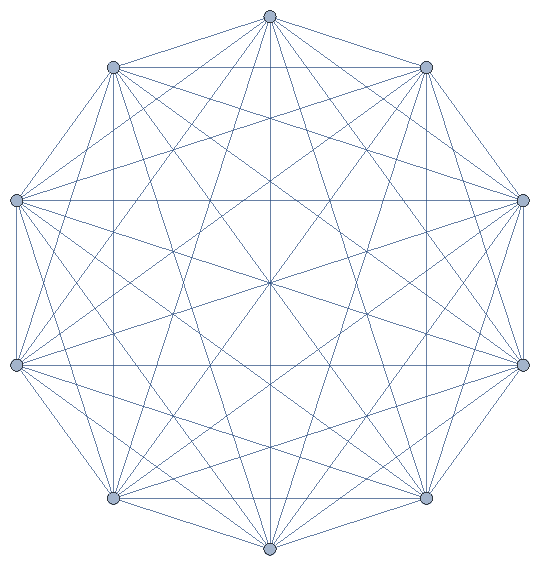
\includegraphics[width=\textwidth]{../ramsza/figs/graph_complete.pdf}
    \caption{Regular graph with \(n = 10\) vertices}
    \label{fig:graphsa}
  \end{subfigure}
  \hfill
  \begin{subfigure}[t]{0.40\textwidth}
    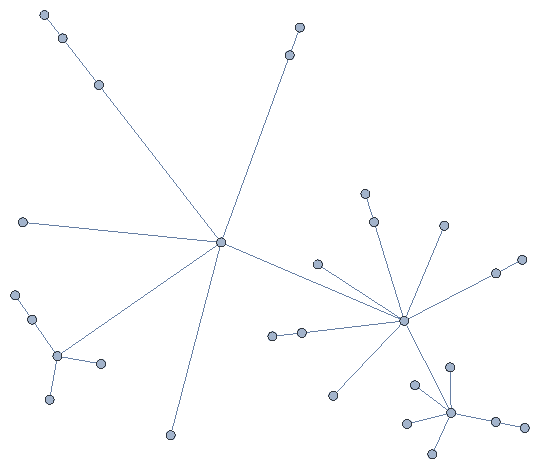
\includegraphics[width=\textwidth]{../ramsza/figs/graph_ba.pdf}
    \caption{BA graph with \( n = 30 \) and \( k = 1\)}
    \label{fig:graphsb}
  \end{subfigure}
  
    \begin{subfigure}[t]{0.40\textwidth}
    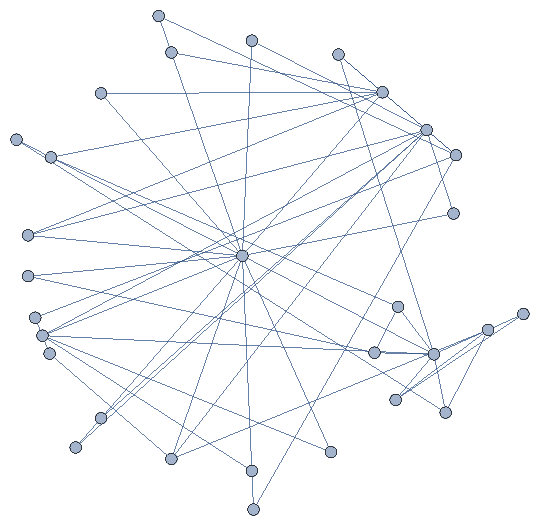
\includegraphics[width=\textwidth]{../ramsza/figs/graph_ba_a.pdf}
    \caption{BA graph with \( n = 30 \) and \( k = 2\)}
    \label{fig:graphsc}
  \end{subfigure}
  \hfill
  \begin{subfigure}[t]{0.40\textwidth}
    
\includegraphics[width=\textwidth]{../ramsza/figs/empty.pdf}
  \end{subfigure}
  
  \captionsetup{margin=10pt,font=small,labelfont=bf,width=.8\textwidth}

  \caption[Exampls of graphs]{Example of regular and BA graphs. \textit{Source:} own calculations}\label{fig:graphs}
\end{figure}

Since in an undirected graph edges represent relations with no regard to their direction, we can denote the relation between vertices $a$ and $b$ either as \(\{$a,b$\}\) or \(\{$b,a$\}\). As an example of an undirected graph, we can think of a graph in which vertices represent humans and edges represent relations between humans, e.g., being friends or connected in a given social network. 

Since these relationships work both ways (if subject \( a\) is a friend of subject \( b\), it implies that subject \(b\) is a friend of subject \(a\)), we only need to use a set \(\{a, b\}\) to denote an edge. We do not use directed graphs in this paper. Henceforth, as a graph, we refer to an undirected graph. 

\subsection{Vertex neighborhood}

Let us define a neighborhood of a vertex in a graph. The neighborhood of vertex $v$ in a graph $G$ is a set of vertices adjacent to the vertex $v$. We call two vertices adjacent when they are connected. The graph induced by a neighborhood of \( v \) is called a neighborhood graph. This concept is crucial for our work because it will allow us to identify all of the vertices able to engage in a game with a previously chosen player. 

\subsection{Degree distribution}

The degree of a vertex $v$ is a number of all vertices connected to the $v$. The important characteristic of a graph is its' degree distribution. The degree distribution is the probability distribution of degrees in a graph. This characteristic varies throughout the different types of graphs. For a regular graph, it is a single value with the probability of 1 because, in a regular graph, all of the vertices have the same degree. Figure~\ref{fig:graphsa} show an example of a regular graph. 

\subsection{Scale-Free Networks}

In our work, we use a type of graph called Scale-Free Network. This type of graph is generated according to the Barabasi-Albert Model, cf.~\cite{albert2002statistical}. The scale-free networks are built in a sequence of steps. We start with a single vertex and, in each step, add a single vertex. The new vertex is connected to the previous vertices with the probability proportional to the vertices' degrees. More precisely, the probability of attaching a new vertex to an already existing vertex \(v\) is given as:
\[ 
p_v = \frac{k_v}{\sum_{j} k_j},
\]
where $k_v$ is a degree of vertex $v$ and $\sum_{j} k_j$ is a sum of degrees of all existing nodes (which, since our graph is an undirected graph, is equal to twice the amount of existing edges). 

This rule favorites the vertices with higher connectivity and causes the graph to have so-called hubs. A hub is a term for a vertex with a considerably higher degree than other vertices. Thanks to this rule, the degree distribution of a graph is given by the formula:
\[
P(k) \backsim k^{-3}.
\]
Figures~\ref{fig:graphsb}--\ref{fig:graphsc} show example of scale-free networks. More precisely, figure~\ref{fig:graphsb} shows an example of a scale-free network built by adding only one edge at every step. Figure~\ref{fig:graphsc} show an example of a scale-free network created by adding two edges at every step. 


% --- chapter ---------------------------------------------------------
\clearpage
\section{Cooperation among the players}\label{sec:coop}

This chapter aims to apply the previously described game theory concepts to the cases used in the simulations. It means that we tell of the PD and SD games and then analyze them. We pay close attention to the parametrizations of the games and how they influence both their solutions (Nash equilibriums) and the eagerness to cooperate among the players.
We also introduce the concept of games played throughout the population of players on preferential attachment graphs and the learning mechanisms in such games. 

\subsection{A brief description of Snowdrift and Prisoners Dilemma games}

\paragraph{Prisoners Dilemma Game.} The Prisoners Dilemma game is a widely known problem in game theory and decision analysis. It shows situations in which the outcome is not optimal, even though players act in their own best interest. In the scope of our analysis, it is essential to note that in the PD game, the best strategy is to defect, regardless of the opponent's choice. The game is parameterized as follows:
\begin{center}
\begin{game}{2}{2}
  & $Cooperate$    & $Defect$    \\
$Cooperate$ & $R,R$ & $S,T$  \\
$Defect$ & $T,S$ & $P,P$
\end{game}
\end{center}
where the values are given as follows:
\[
\begin{aligned}
T &= b > 1, & R &= 1, \\
P &= 0, & S &= 0, \\
1 &< b \le 2. 
\end{aligned}
\]
We see that the above restrictions order the parameters as follows:
\[
T > R > P = S .
\]

\paragraph{Snowdrift Game.} The Snowdrift game represents a metaphor for cooperative interactions between players. Contrary to the PD game, the Snowdrift game stimulates cooperative behavior amongst players. It doesn't make the deflection strategy inapplicable, but the game's payoffs encourage cooperative behavior more than the payoffs of the PD game. The optimal strategy is to cooperate when the other defects and to defect when the other cooperates. The game is parametrize as follows:
\begin{center}
  \begin{game}{2}{2}
    & $Cooperate$    & $Defect$    \\
  $Cooperate$ & $R,R$ & $T,S$  \\
  $Defect$ & $S,T$ & $P,P$
  \end{game}
  \end{center}
where the parameters' values are:
\[
  \begin{aligned}
  T &= \beta > 1 , &  R &= \beta - \frac{1}{2} ,\\
  S &= 1 - \beta , &  P &= 0. 
  \end{aligned}
\]
We see that the above restrictions order the parameters as follows:
\[
 T > R > P > S .
\]

To represent the cost-to-benefit ratio of mutual cooperation we define $r$ as follows: 
\[
  r = \frac{1}{2\beta-1},
\] with $0<r\leq1$ cf.~\cite{santos2005scale}.

\subsection{Analysis of PD and SD games}

\paragraph{Nash equilibria.}

Since our work covers 20 parametrizations for each game, we discuss Nash equilibrium in those games for the two farthest parametrizations. Let us start with a description of the Prisoners Dilemma game. For the smallest possible value of parameter $b$ equal to $1$, we represent the game as follows:

\begin{center}
  \begin{game}{2}{2}
    & $Cooperate$    & $Defect$    \\
  $Cooperate$ & $1,1$ & $0,1$  \\
  $Defect$ & $1,0$ & $0,0$
\end{game}
\end{center}

Player one chooses the row strategy and player two chooses the column strategy. In each cell of the matrix, player one's payoff is represented as the left value. 

For the second parametrization of PD we want to show the one with biggest payoffs. The payoff matrix looks like following:

\begin{center}
  \begin{game}{2}{2}
    & $Cooperate$    & $Defect$    \\
  $Cooperate$ & $1,1$ & $0,2$  \\
  $Defect$ & $2,0$ & $0,0$
\end{game}
\end{center}

For both of these parametrizations, we obtain at least one Nash equilibrium. In the first case, we get two Nash equilibriums. One for strategy profile $\{Cooperate, Cooperate\}$, the other for $\{Defect, Defect\}$. In both cases, the Nash equilibrium is weak, hence the players are indifferent to the choice of their strategy.
In the case of $b = 2$, we have only one Nash equilibrium for the strategy profile of $\{Defect, Defect\}$. Moreover, in this case, the strategy $Defect$ is a weakly dominant strategy for both players. 

The term \enquote{strictly (weakly) dominant strategy} refers to a situation in which one of the player's strategies gets him higher (or at least the same utility) as any other strategy for all of the possible strategy profiles cf.~\cite{wozny2012lecture}. 

To parametrize the second game --- SD, we vary the $r$ parameter. To present the payoff matrix, we need to manipulate formula 
\[
  r = \frac{1}{2\beta -1},
\] 
so that we can easily calculate the $\beta$ value. It's given as follows: 
\[
  \beta = \frac{1-r}{2r}.
\] The lowest value of $r$ is supposed to be as close to $0$ as possible. For this paper, we use the smallest value of $r$ equal to $10^{-5}$ and consider it a good enough approximation. For the said value of $r$, we write the payoff matrix as follows:

\begin{center}
  \begin{game}{2}{2}
    & $Cooperate$    & $Defect$    \\
  $Cooperate$ & $4999,4999$ & $4999.5,4998.5$  \\
  $Defect$ & $4998.5,4999.5$ & $0,0$
\end{game}
\end{center}

We conclude that, for this game, both players have a strictly dominant strategy --- $Cooperate$. Therefore we also get a strict Nash equilibrium for the strategy profile of $\{Cooperate, Cooperate\}$. 

As the $r$ parameter reaches its highest value --- $1$, the value of $\beta$ approaches to $0$. Thus, the payoff matrix looks as follows:

\begin{center}
  \begin{game}{2}{2}
    & $Cooperate$    & $Defect$    \\
  $Cooperate$ & $-\frac{1}{2},-\frac{1}{2}$ & $0,-1$  \\
  $Defect$ & $-1,0$ & $0,0$
\end{game}
\end{center}

The SD game with those payoffs also favorites the $Cooperate$ strategy because this strategy is dominant (even though it is only weakly dominant).

There are two Nash equilibriums in this game. One occurs for the strategy profile of $\{Cooperate, Cooperate\}$, and the other is for strategy profile $\{Defect, Defect\}$. Even though the Nash equilibrium for $defection$ gives higher payoffs, players are more likely to $cooperate$ because of this strategy dominance.

% --- Gry na grafach losowych -----------------------------------------

\subsection{Games on graphs}


The model for the population of players in this paper is a previously described Barabasi-Albert model (i. e. Scale-Free Network). This model is generated randomly, with set parameters, for each simulation. Players occupy vertices of these graphs. Two players are able to engage in a game when they are connected --- there must exist a vertex between two vertices. 

We use this type of graph because it is considered the best description of complex networks of agents in many areas of study --- e. g. biology, sociology, and economics \cite{volchenkov2002epidemic}. The most important characteristic of those graphs is that there exist \enquote{hubs} --- vertices with a considerably higher degree than the average. Those differences in vertices' degrees might be interpreted as inequalities among the players. 

\subsection{Learning procedure in population games}

The main objective of this paper is to present the proportion of $cooperate$ and $defect$ strategies for both PD and SD games. To do so, we must introduce the concept of learning in population games. This idea is based on the hypothesis that players can \enquote{adapt} to the games' rules by changing their strategy. For the description of this procedure we rely on the \cite{santos2005scale}. 

The incentive for the players to alter their strategies is represented by their accumulated payoff. By the accumulated payoff, we mean the sum of all payoffs obtained by the player in the current simulation. 
After all edges (pairs of connected players) engage in a single round of given game, one player is chosen arbitrarily --- let us call him player one. 

Then of all his neighbors we randomly select one with a different strategy (i. e. if player one's strategy is $cooperate$, we select a neighbor with a strategy $defect$) --- let us name him player two.

We determine which strategy is to be altered. We do this by comparing their accumulated payoffs --- the player with a greater value will try to \enquote{take over} the other player and impose his strategy onto him. This procedure is nonetheless not definite and comes with a given probability. 

Let us introduce an example of player $1$ taking over player $2$. The probability of the transition is given as follows:
\[
  p_t = \frac{P_1-P_2}{Dk_>},
\]
where $p_t$ is the probability of transition, $P_1$ and $P_2$ are accumulated payoffs of player one and player two, respectively. Parameter $D$ depends on the type of game that is being played --- generally speaking it is the biggest obtainable payoff in a single round of a game, decreased by the $S$ or $P$ paramter for PD and SD, respectively. Therefore for both PD and SD, it is equal to the parameter $T$, because both $S$ and $P$ parameters are equal to $0$. The $k_>$ parameter is the greater value between both players' number of neighbors.
If the transition is sucessful we adjust the vector of strategies by alterint the responding element. 
% --- chapter ---------------------------------------------------------
\clearpage
\section{Algorithms and simulations}

This chapter contains a description of the functions, algorithms, and procedures used to conduct the necessary simulations. We must remold all mathematical concepts and ideas presented beforehand into a functioning code that allows us to produce analyzable results. The code is written in the julia language to obtain high efficiency while easy to follow and readable.

The description of the algorithm used in the paper \cite{santos2005scale} is unclear, therefore insufficient for exact replication. As a result, we may create a couple of different procedures based on different interpretations of said description. The algorithm described in this paper is the simplest and easiest to carry out. 

\subsection{Simulations description}

Because of the nature of this paper, our simulations must be conducted in a strict accordance with the methods outlined
in \cite{santos2005scale}. Therefore it is only natural that we must follow each step with the utmost care and diligence. We must conduct 100 simulations for each parametrization. Each simulation is performed following those steps:
\begin{enumerate}
  \item Setting up the parameters which are needed to create SF NOCs (such as the number of final vertices (population size), the average connectivity, etc.).
  \item Choosing the parameters, e. g. the payoffs, of the game which is to be simulated (either PD or SG).
  \item Creating the randomly generated SF NOC (we use Barabasi - Albert model to do that). The SF NOC must be created in compliance with preferential attachment and 
  growth rules.
  \item Randomly distributing strategies amongst the population. Each vertex (player) can either get a $cooperate$ or $defect$ strategy.
  \item Every edge (i. e. two connected players) engage in a round of a given game --- this procedure is one \enquote{generation}. One simulation consists of 2100 generations. After each generation an attempt is made to alter one of the players strategy.
  \item We collect results (equilibrium frequencies of cooperators and defectors) by averaging over the last 100 generations.
\end{enumerate}

\subsection{Functions}

In order to perform necessary calculations I had to define the following functions:

\begin{enumerate}
  \item \lstinline+Transform+ --- This function is used to map strategies onto a vector of arrays. As an input this function takes one of the edges of a SF NOC,
   as an output it returns a vector of length two (two vertices connected with an edge).
  \item \lstinline+Strat+ --- This function is used to map previously distributed strategies onto a vector of edges. As an input it takes an edge and as an output
   it returnes a vector of length two (two strategies previously attributed to the vertices).
  \item \lstinline+Games+ --- This function is used to evaluate the results of games played between players (vertices connected with an edge). As an input this function
   takes a vector of edges, vector of strategies and a vector of accumulated payoffs. It returns an adjusted vector of accumulated payoffs.
  \item \lstinline+CheckStrat+ --- This function fulfills a number of tasks. It takes as an input a randomly chosen vertex, vector of strategies, vector of accumulated
  payoffs, and the SF NOC. It identifies all neighbors of the previously mentioned vertex, then shuffles them, and then looks for a neighbor
  with a different strategy. Then it proceeds to change the strategy of the vertex with lower accumulated payoffs. The probability of the transition 
  is described in section 4.4. \todo{Jak dodać odnośnik do podrozdziału 4.4?} 
\end{enumerate}

\subsection{Description of the algorithm}

The main algorithm is the fundamental element of this paper. It consists of 3 nested loops executing instructions necessary to conduct simulations, on which our research is based. I will be describing those loops in an inside-out order. 

The first loop is responsible for evaluating the results of the games, potentially changing the strategies of players, and keeping track of the proportion of the strategies used by players. To run properly, it requires previously set parametrization and a set of edges of the Barabasi-Albert graph. 

As a result, it produces a vector of length 100 in which elements are proportions of coop/def strategies, measured after each generation (2001--2100) in the population of players. 

This loop is repeated 2 000 times, which gives us a total of 2~200~000 generations for one Barabasi-Albert graph parametrization for a given game.
The loop itself operates as follows:

%\begin{enumerate}[noitemsep]
%  \item Each pair of connected players (vertices of a graph) engage in a single round of a given game. It means that function GAMES is applied throughout the entire array of edges, adjusting their accumulated payoffs.
%  \item One player is chosen randomly.
%  \item An attempt to change strategy is being embarked on. It indicates that the function CHECKSTRAT is applied to the player chosen in the previous step.
%  \item If the current iteration is higher than 1000, it calculates the share of cooperators in the entire population and then passes it onto a corresponding value of a vector TRACK.
%  \item After 1~100 iterations (generations), it ends, and then the next iteration of the outside loop is triggered.
%\end{enumerate}

\begin{algorithm}[H]
  \KwData{Barabasi-Albert Model, array of edges, array of strategies, array of accumulated payoffs (initially equal to 0), empty vector of length 100, parametrization of the games}
  \KwResult{Vector of length 100 containing coop/def proportion for the population}
  initialization \;
  \For{k in generations}{

    \eIf{k is greater than $1$}{
      Adjust the array of strategies associated to players. \;
    }

    Play a single round of a given game between all possible pairs of players by applying function \lstinline+games+ on a vector of edges. \;
    Randomly choose one vertex.\;
    Attempt to change the strategy of the previously chosen player (or one of his neighbors) by applying function \lstinline+CheckStrat+. \;
   \eIf{k is greater than the number of generations minus $100$}{
    Evaluate the coop/def proportion in the entire population \;
    Save the result to the appropriate value of a vector. \;
    }{}
  }
\caption{The inner loop}
\end{algorithm}
 
The outer loop to the one described above is responsible for \enquote{resetting} the Barabasi-Albert graph. Since separate simulations are supposed to be carried out on a randomly generated SF NOC (but with the same parametrization), we need to conduct 100 of them (for each payoff parametrization); this loop is an indispensable element of the algorithm. 

The crucial fact to note is that this loop is also responsible for creating an object named \lstinline+ArrPath+ --- vector of length 100, used to store the results of the simulations.

The procedure followed by this loop is as shown below:

%\begin{enumerate}
%  \item It generates the random Barabasi-Albert graph with N vertices and average connectivity equal to Z. Both parameters are chosen deliberately at the beginning of the code.
%  \item The next step is constructing an array of strategies. This array is of length 1000 (number of players). The strategies are represented by numbers 1 (cooperation) and 2 (defection). The choice of these numbers is strict because later on, we use them to index the payoffs matrix.
%        The process of creating such an array is following:
%        \begin{enumerate}
%          \item Creating two vectors of length 500, one filled with ones, and one filled with twos.
%          \item Concatenate those two vectors to get a vector of length 1000.
%          \item Shuffle the values in a vector and save them as STRATEGIES.
%        \end{enumerate}
%  \item For the inner loop to conduct games, we need to transform our SF NOC into two arrays --- one containing edges (tuples of players) and the other containing strategies for each edge. To achieve this, we apply the following steps:
%        \begin{enumerate}
%          \item We use function COLLECT on the function EDGES used on the Barabasi-Albert model, which results in an iterable, however not easily callable, array of edges.  
%          \item Then we map a function TRANSFORM onto the previously obtained object. This produces us an array of tuples, each tuple representing one edge.
%          \item Lastly, we map function STRAT onto an array of tuples representing the edges.
%        \end{enumerate}
%  \item The array of accumulated payoffs is created --- initially with all values equal to zero (after each game, the results are added to the corresponding values in this array).
%  \item A global variable is created. This variable is named TRACK and it is a vector of length 100. This vector is used by the inner loop to store the proportion of cooperators in the population.
%  \item The final step before triggering the inner loop is creating ARRPATH, which will be used to store 100 TRACK variables. If it is the first iteration of this loop, we create a global variable named ARRPATH, which is an array. If, on the other hand, it is not the first iteration, we are using the function PUSH! to 
%        add the next TRACK to our existing array. 
%\end{enumerate}

\begin{algorithm}[H]
  \KwData{Barabasi-Albert parametrization}
  \KwResult{Scale-Free Network built by Barabasi-Albert Model, list of edges, list of strategies, vector of accumulated payoffs, ArrPath --- an array of length 100 storing results of the simulations}
  initialization \;
  \For{j in simulations}{
   Create a Scale-Free Network by using the Barabasi-Albert model with previously set parameters.\;
   Create an array of length equal to the number of players, containing their strategies. \;
   Extract an array of edges from a previously created graph by mapping function \lstinline+transform+ onto a list of edges. \;
   Produce an array of tuples representing strategies for every player by mapping a function \lstinline+strat+ onto an array of edges. \;
   Create an array of accumulated payoffs (initially filled with zeros). \;
   Generate a vector of length 100 filled with zeros, called \lstinline+track+. This vector will be later on used to store coop/def proportions. \;
   \eIf{j equals to 1}{
    Create an object called \lstinline+ArrPath+ with one element equal to \lstinline+track+. \;
    }{
    Merge the current \lstinline+track+ with \lstinline+ArrPath+. \;
   }
   Initiate the inner loop described above. \;
  }
  \caption{Second loop}
 \end{algorithm}

 The outer loop is in charge of setting the parametrs of the games. Since we want to obtain 20 data points for a single Barabasi-Albert Model parametrization, we need to iterate 20 times executing the previously described loops. The payoffs for our games are 
 of range $[1,2)$ and $(0,1]$ for PD and SD, respectively. We need to divide the span (which is equal to 1 in both cases) by the number of data points, and we gain a result of 0.05. 
 
 Thus each iteration adds 0.05 to the payoffs of both games. Furthermore, this loop is also responsible for creating and object called \lstinline+DataToSave+ that will store our results. Atfer the loop ends, the \lstinline+DataToSave+ object is saved into the local repository.
 
 \begin{algorithm}[H]
  \KwData{None}
  \KwResult{Parametrization for the games, \lstinline+DataToSave+ --- an array of vectors that will be used to store and ultimately save our results.}
  initialization\;
  \For{i in number of parametrizations}{
   \eIf{i is equal to 1}{
    Create an array of length 20 --- \lstinline+DataToSave+. ;
    }{
    Store the current \lstinline+ArrPath+ as a value of \lstinline+DataToSave+. \;
   }
   Set up payoffs of the games based on the current iteration. In each iteration, add 0.05 to the current values of the payoffs. \;
   Create a matrix of payoffs for the games with current parametrization. \;
   Initiate the second loop. \;
   Save \lstinline+DataToSave+ to the local repository. \;
  }
  \caption{The outer loop}
 \end{algorithm}
 
% --- chapter ---------------------------------------------------------
\clearpage
\section{Results and discussion}

In this chapter, we describe the data manipulations and methods used to transform our results into a readable and easy-to-present format. Then, we describe and discuss our results. We compare them to those presented in \cite{santos2005scale} and discuss the eventual discrepancies. 

\subsection{Format of obtained data}

The data we obtain is in form of a vector of length 20 --- let us call it $P$. Each value of this vector is another vector of length 100, containing vectors of length 100. Therefore it can be easily transformed into a vector of matrices of size $100 \times 100$. We interpret row number as a simulation's number (for each parametrization we performed 100 simulations) and column number as a generation's number from which the proportion is extracted. Therefore, we can present results for a single games' payoffs parametrization as follows:
\[
R = \begin{bmatrix} 
    r_{11} & \dots & r_{1M} \\
    \vdots & \ddots & \vdots \\
    r_{N1} &  \dots      & r_{NM} 
    \end{bmatrix}
,\]
where $R$ is a matrix of the results, $r_{NM}$ is a coop/def proportion after $2000 + M$ generations in the $N$-th simulation. Now, we may denote $P$ as:
\[
  P = (R_1, \dots, R_{20}),
\]
where $R_i$ is the matrix of results for the \(i\)-th iteration of the parametrization loop.

To present our data as a plot, we bring the $R_i$ matrices into a single value. We do that by simply averaging all matrix elements. The formula is as follows:
\[
  \frac{\sum_{k=1}^{N}\sum_{j=1}^{M} r_{kj}}{N \cdot M} .
\] 

Applying the above procedure to our vector \( P\) results in gaining 20 data points, and allows us to produce one plot for each Barabasi-Albert Model parametrization. Since we have three such parametrizations for each game, we gain 6 plots of coop/def tracks. We've decided to group them in regard to games so that they could be easily compared. 

\subsection{Discussion}

The results seem to agree with the general intuition concerning the game theory. As we analyzed PD and SD games in section~\ref{sec:coop}, we highlighted the Nash equilibria and optimal, in this sense, strategies. 

For the PD game, we demonstrated that for the lowest value of the parameter $b$ (equal to \( 1\) ), players are indifferent to the choice of their strategies. 

Figure~\ref{fig:resa} shows cooperation profiles for a grid of values of the parameter \( b\). It is clear, that for \( b\) close to \(1\), the share of cooperators is close to \(1/2\). 

We may observe that on the Figure~\ref{fig:resa}, the share of cooperators for $b=1$ is close to $0.5$. As the value of $b$ increases, we can see that the average share of cooperators is decreasing. This is also a reasonable result --- $b$ parameter influences the dominance of $Defect$ strategy amongst the population of players. Thus, the higher the $b$ parameter is, the more competitive the $defect$ strategy becomes. 

We may also observe that as the main Barabasi-Albert model's parameter --- average connectivity increases, the players tend to prioritize the dominant strategy more frequently. 

As far as the SD goes, we obtained the quite opposite results. Since the main parameter --- $r$ represents the cost-to-benefit ratio of mutual cooperation, we expect our curve to start off high and then decline as the $r$ increases. 

We can see from the plot \ref{fig:resb} --- that it is the case. Moreover, we can conclude that with the increase in average connectivity, the proportion of coop/def strategies seems to react slower to the adjustments of $r$. This means that if players can engage in more games during each generation, they are more likely to change their strategies to $Cooperate$ even for a higher cost-to-benefit ratio. 

\todo{Tutaj wpisujemy uzyskane wyniki oraz dyskutujemy je, np. porównujemy do wyników z oryginalnego artykułu.}

 \begin{figure}[hbt]
  \centering
  \begin{subfigure}[t]{0.45\textwidth}
    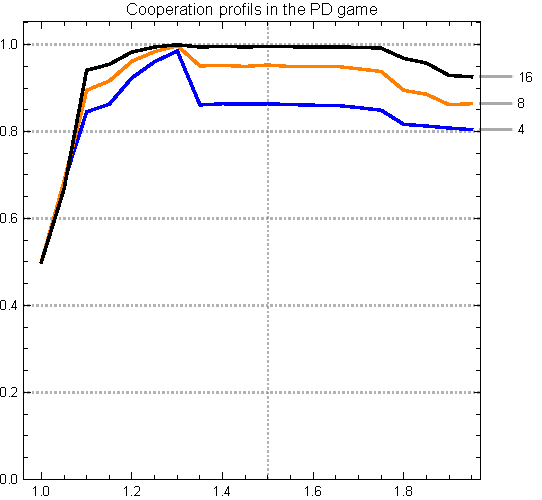
\includegraphics[width=\textwidth]{../ramsza/figs/PD_profiles.pdf}
    \caption{PD game}
    \label{fig:resa}
  \end{subfigure}
  \hfill
  \begin{subfigure}[t]{0.45\textwidth}
    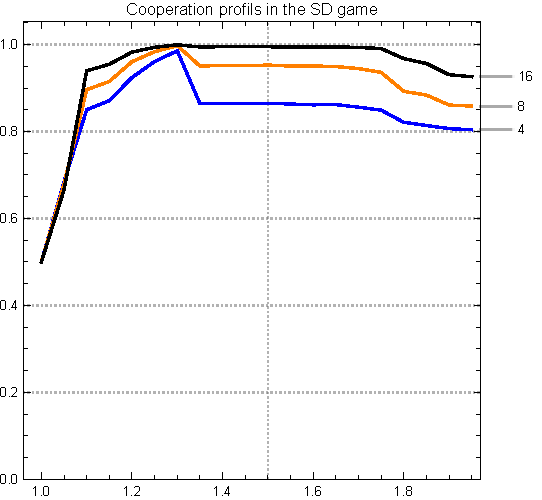
\includegraphics[width=\textwidth]{../ramsza/figs/SD_profiles.pdf}
    \caption{SD game}
    \label{fig:resb}
  \end{subfigure}

  
  \captionsetup{margin=10pt,font=small,labelfont=bf,width=.8\textwidth}

  \caption[Cooperation profiles]{Cooperation profiles for the PD and SD games. \textit{Source:} own calculations}\label{fig:res}
\end{figure}

% --- chapter ---------------------------------------------------------
\clearpage
\section{Conclussions}

Throughout the course of this paper, we have managed to accomplish --- to some extent, both of the goals set in the first chapter. We produced results that comply with the game theory intuition for the analyzed games. We also provided an replicable and easy to use code writeen in julia language. 

Those results do not however match completely the ones in \cite{santos2005scale}. Our main concern is that the high cooperation rate presented in the mentioned paper is neither obtainable with the procedure we used nor intuitive (since PD favorites defection strategy over the coop). Our procedure is of course debatable in terms of the number of conducted generations (we used $2 100$ generations instead of $10 100$). However, we can't think of any reason why increasing the number of generations would change the results so dramatically. 

The results for the SD game are, to some degree, similar to those obtained in the comparative article. It is only natural for the cooperation ratio to be high in a game that heavily favorites the $Cooperate$ strategy. Moreover, we can conclude from \ref{fig:resb} that increasing the avarage connectivity of the graphs that under 

%\begin{table}[hbt]
%  \centering
%\end{table}
%% --- chapter ---------------------------------------------------------
%\clearpage
%\section{Basic things}
%
%\subsection{Compiling \LaTeX files}
%
%The \verb+.tex+ file is just a plain text file. It contains the \LaTeX formatting codes together with the content of a paper. To get a \verb+.pdf+ file you have to compile the \verb+.tex+ file using a sequence \verb+pdflatex+, \verb+biblatex+, \verb+pdflatex+, \verb+pdflatex+. This sequence is a default in most editors designed for use with \LaTeX.
%
%\subsection{Basic formatting for a text}
%
%Paragraphs are coded by an empty line. That is is you want to start a new paragraph it is enough to leave an empty line and start typing like that:
%\begin{verbatim}
%This is the first paragraph.
%
%This is the next paragraph.
%\end{verbatim}
%
%Everything about the paragraph is formatted for you including all indents and spacings. Again, you don't have to take care of it manually.
%
%Basic text formatting, e.g. bold face and italic, is achieved with the following commands: \verb+\textbf{}+, \verb+\textit{}+, \verb+\underline{}+, producing \textbf{text}, \textit{text}, \underline{text}. I suggest not overusing those commands!
%
%Alignment is done through environments \verb+center+, \verb+flushleft+ and \verb+\flushright+ giving the following examples.
%
%\begin{center}
%  This is centered.
%\end{center}
%
%\begin{flushleft}
%  This is aligned to the left.
%\end{flushleft}
%
%\begin{flushright}
%  This is aligned to the right. 
%\end{flushright}
%
%In other environments it is possible to use \verb+\centering+ to center content of that environment (like in \verb+figure+ or \verb+table+ environments).
%
%\subsection{Fonts and fonts' sizes}
%
%You do not change fonts and fonts' sizes! Technically it can be done but I will reject this.

%% --- chapter ---------------------------------------------------------
%\clearpage
%\section{Mathematics}
%
%This is testing footnotes\footnote{This is a footnote. We can put some math here \( x^2 - f(x) = g(x^2) \) which is not encouraged but sometimes necessary. The other thing we can do is to put here an URL \url{https://tex.stackexchange.com/questions/249415/set-font-size-for-footnotes}. }.
%
%\subsection{Basic mathematics}
%
%There are two types of mathematics inside a \LaTeX{} document. The first one is the in-line mathematics and the displayed mathematics. The first one looks like this: \( F(x) = \int_{-\infty}^{x} f(\omega) d\omega \) with the code looking like this: \verb!\( F(x) = \int_{-\infty}^{x} f(\omega) d\omega \)!. The displayed mathematics looks like that
%\[
%F(x) = \int_{-\infty}^{x} f(\omega) d\omega
%\]
%with the code
%\begin{verbatim}
%\[
%F(x) = \int_{-\infty}^{x} f(\omega) d\omega
%\]
%\end{verbatim}
%As you can see the same code is formatted differently depending on the type of mathematics.
%
%\subsection{Referencing mathematics and other things}
%
%To reference mathematics (only displayed formulas) you use the \verb+equation+ environment with a \verb+\label{}+ within. The reference is done through the \verb+\ref{}+ command. The example is
%\begin{equation}
%\label{eq:this-is-very-important-equation}
%F(x) = \int_{-\infty}^{x} f(\omega) d\omega.
%\end{equation}
%To reference the equation you use the \verb+\ref{}+ command giving (\ref{eq:this-is-very-important-equation}). The \verb+\label{}+ / \verb+\ref{}+ pair works for anything that can be referenced.
%
%\subsection{Some more mathematical formulas}
%
%Here are slightly more complex formulas. Let \( A  \) be a matrix
%\[
%A =
%\left(
%\begin{bmatrix}
%1                   & \alpha^2       \\
%2                   & \sqrt{\pi} - \log(x-\sin(y))
%\end{bmatrix}^{2}
%- 
%\begin{bmatrix}
%1                   & f(x)           \\
%2                   & g(y)
%\end{bmatrix}
%\cdot
%\begin{bmatrix}
%x                                    \\
%y
%\end{bmatrix}
%\right),
%\]
%where
%\[
%f(x) = 
%\left\{
%  \begin{aligned}
%    \frac{1}{x}     & \quad \text{for \(x<-\frac{1}{2}\),} \\
%    \frac{1}{1+x^2} & \quad \text{for \(x \geq -\frac{1}{2}\)}
%  \end{aligned}
%\right.
%\]
%and
%\[
%g(y) = \sin\left(\frac{\mathrm{\mathbf{E}}(X)}{\cos(y) + \log(y)}\right), 
%\quad\text{where \( X \sim \mathrm{N}(0, \sigma)  \).}
%\]
%
%It is very easy to typeset a normal form game. Below is an example of such a game. 
%
%\begin{game}{3}{3}
%    & $L$    & $M$    & $H$    \\
%$L$ & $16,9$ & $3,13$ & $0,3$  \\
%$M$ & $21,1$ & $10,4$ & $-1,0$ \\
%$H$ & $9,0$  & $5,-4$ & $-5,-15$
%\end{game}
%
% --- chapter ---------------------------------------------------------
%\clearpage
%\section{Figures and tables}
%
%Both figures and tables use the same ideas. To insert a table you use the \verb+table+ environment. This is an example of a simple table.
%
%\begin{table}[hbt]
%  \centering
%
%  \captionsetup{margin=10pt,font=small,labelfont=bf,width=.8\textwidth}
%
%  \caption[Short name for a table]{This is an example of a table.}
%  \label{tab:exceptional-table}
%
%\vspace*{2ex}
%
%  \begin{tabular}{lccc}
%    Name        & property 1 & property 2 & property 3 \\ \hline
%    Michael     & 23         & 34         & --         \\
%    John        & 34         & --         & 28         \\
%    Mr. Niceguy & 123        & 231        & 312        \\ \hline
%  \end{tabular}
%\end{table}
%
%Table~\ref{tab:exceptional-table} is a very simple table and much more is possible.
%
%To insert a figure you need to have a figure. In the catalog there are two figures and the following is an example of the \verb+figure+ environment.
%
%\begin{figure}[hbt]
%  \centering
%
%  \begin{subfigure}[t]{0.45\textwidth}
%  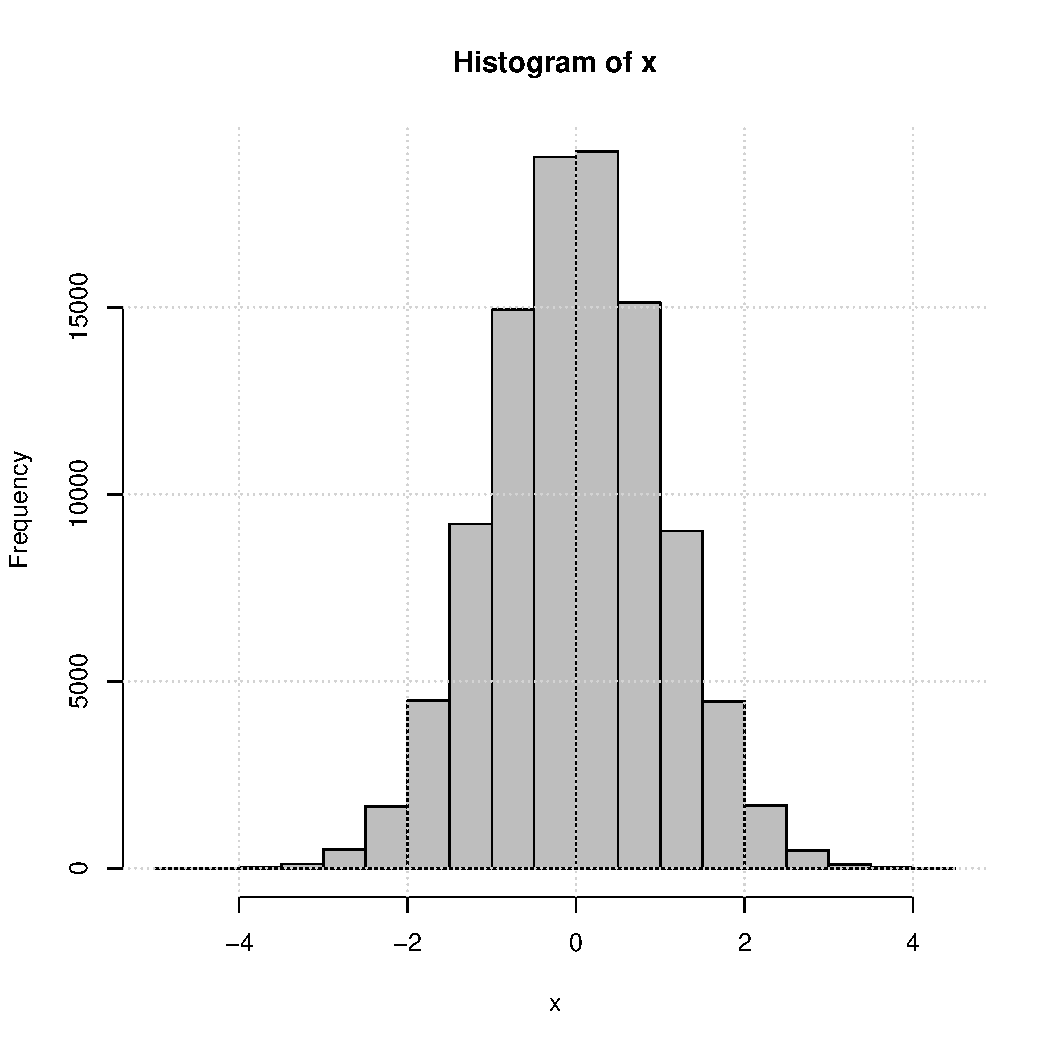
\includegraphics[width=\textwidth]{./figure-1}
%  \end{subfigure}
%
%  \captionsetup{margin=10pt,font=small,labelfont=bf,width=.8\textwidth}
%
%  \caption[Short name]{This is just an example. \textit{Source:} own calculations.}\label{fig:xxx1}
%\end{figure}
%
%\begin{figure}[hbt]
%  \centering
%  \begin{subfigure}[t]{0.45\textwidth}
%    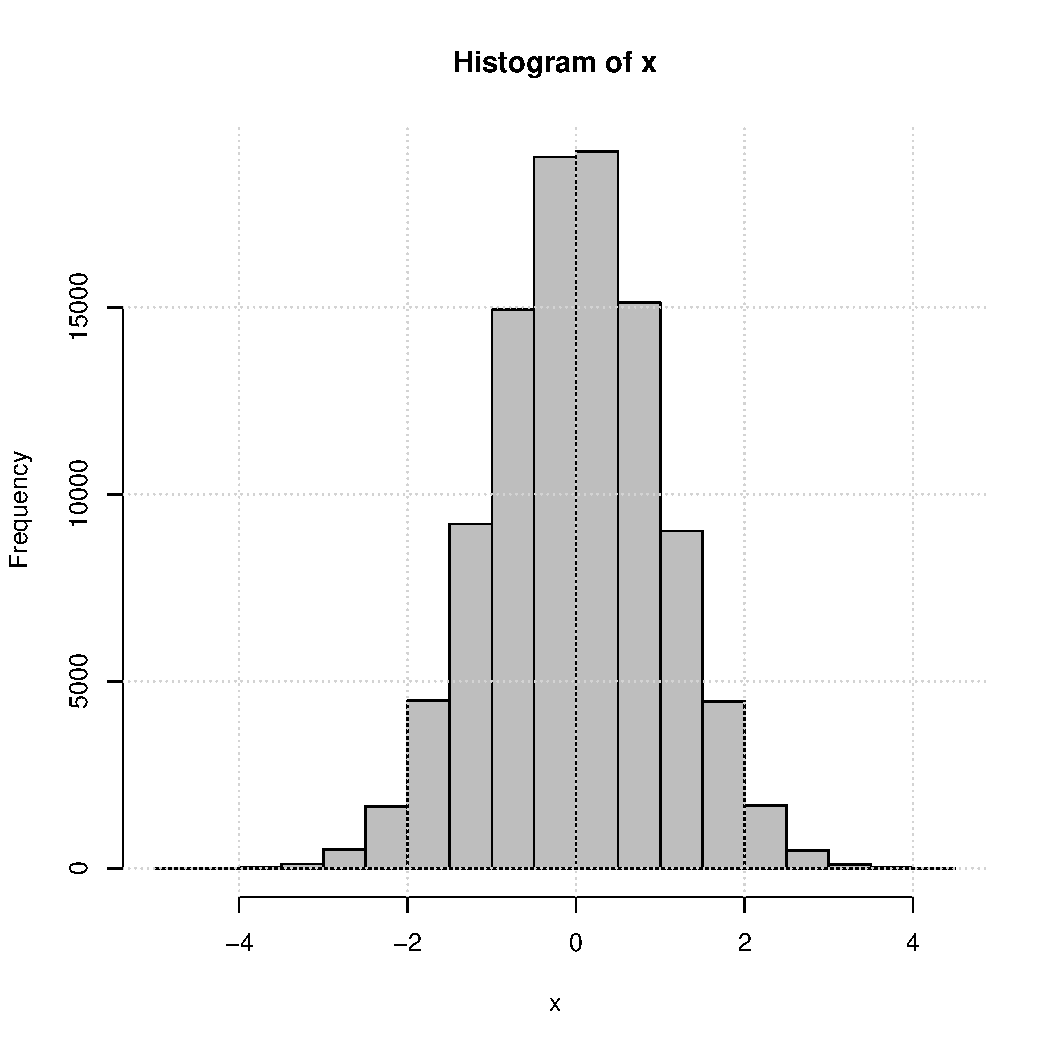
\includegraphics[width=\textwidth]{./figure-1}
%    \caption{This is a caption for the first figure. This caption is wrapped at the right width and the hight is being compensated.}
%    \label{fig:xxxa}
%  \end{subfigure}
%  \hfill
%  \begin{subfigure}[t]{0.45\textwidth}
%    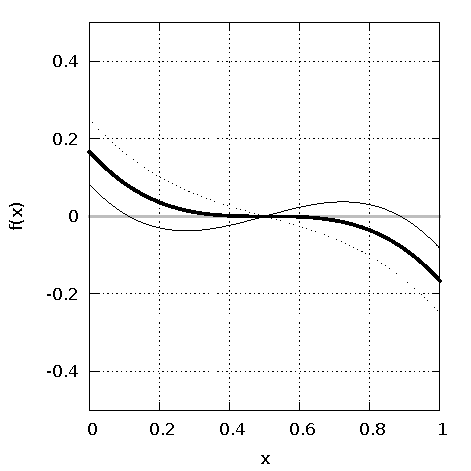
\includegraphics[width=\textwidth]{figure-2}
%    \caption{This is another caption.}
%    \label{fig:xxxb}
%  \end{subfigure}
%  
%  \captionsetup{margin=10pt,font=small,labelfont=bf,width=.8\textwidth}
%
%  \caption[Short caption 2]{This is the main caption and it is below the figures. \textit{Source:} own calculations}\label{fig:xxx}
%\end{figure}
%
%Figure~\ref{fig:xxx} is a slightly more complex than just a simple figure but it is useful to have such template. It is possible to refrence subfigures as \ref{fig:xxxa} and \ref{fig:xxxb}.

%% --- chapter ---------------------------------------------------------
%\clearpage
%\section{Bibliography}
%
%\begin{wrapfigure}{r}{.5\textwidth}
%\centering
%
%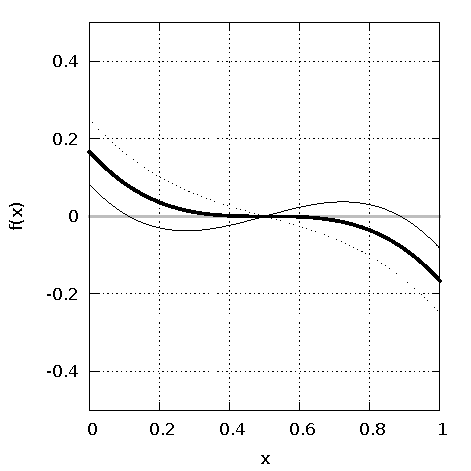
\includegraphics[width=.4\textwidth]{figure-2}
%
%\captionsetup{margin=10pt,font=small,labelfont=bf,width=.42\textwidth}
%
%  \caption[Short caption 2]{This is how one can wrap a text around a figure. \textit{Source:} own calculations}\label{fig:yyy}
%
%
%\end{wrapfigure}
%
%The content for the bibliography is in a different file named \verb+refs.bib+. You can change the name but then you have to change the information in this file from \verb+\bibliography{refs}+ to \verb+\bibliography{new-name}+ where \verb+new-name+ is the name of your file. The file \verb+refs.bib+ contains some examples for books and papers.
%
%The process of citation is simple. The command  \verb+\cite{garland2010}+ gives this \cite{garland2010} and puts all information into the bibliography section  at the end. Everything is sorted and formatted for you so that you don't have to worry about this. An example of a paper with many authors is \cite{benaim2003} or \cite{osborne1998}. 
%
%\begin{longtable}{rrrrr}
%\caption{Binary variables used in the VAR model}\label{tab:1}     \\
%  \hline
% t   & year & elections & crises & tax cuts                       \\ 
%  \hline
%  \endfirsthead
%  \multicolumn{5}{c}%
%{\tablename\ \thetable\ -- \textit{Continued from previous page}} \\
%\hline
%t    & year & elections & crises & tax cuts                       \\ 
%\hline
%\endhead
%\hline \multicolumn{5}{r}{\textit{Continued on next page}}        \\
%\endfoot
%\hline
%\endlastfoot
%  1  & 1961 & 0         & 0      & 0                              \\ 
%  2  & 1962 & 0         & 0      & 0                              \\ 
%  3  & 1963 & 0         & 0      & 0                              \\ 
%  4  & 1964 & 1         & 0      & 0                              \\ 
%  5  & 1965 & 0         & 0      & 1                              \\ 
%  6  & 1966 & 0         & 0      & 0                              \\ 
%  7  & 1967 & 0         & 0      & 0                              \\ 
%  8  & 1968 & 1         & 0      & 0                              \\ 
%  9  & 1969 & 0         & 0      & 0                              \\ 
%  10 & 1970 & 0         & 0      & 0                              \\ 
%  11 & 1971 & 0         & 0      & 0                              \\ 
%  12 & 1972 & 1         & 0      & 0                              \\ 
%  13 & 1973 & 0         & 0      & 0                              \\ 
%  14 & 1974 & 0         & 1      & 0                              \\ 
%  15 & 1975 & 0         & 1      & 0                              \\ 
%  16 & 1976 & 1         & 0      & 0                              \\ 
%  17 & 1977 & 0         & 0      & 0                              \\ 
%  18 & 1978 & 0         & 0      & 0                              \\ 
%  19 & 1979 & 0         & 0      & 0                              \\ 
%  20 & 1980 & 1         & 0      & 0                              \\ 
%  21 & 1981 & 0         & 0      & 0                              \\ 
%  22 & 1982 & 0         & 1      & 1                              \\ 
%  23 & 1983 & 0         & 0      & 0                              \\ 
%  24 & 1984 & 1         & 0      & 0                              \\ 
%  25 & 1985 & 0         & 0      & 0                              \\ 
%  26 & 1986 & 0         & 0      & 1                              \\ 
%  27 & 1987 & 0         & 0      & 0                              \\ 
%  28 & 1988 & 1         & 0      & 0                              \\ 
%  29 & 1989 & 0         & 0      & 0                              \\ 
%  30 & 1990 & 0         & 0      & 0                              \\ 
%  31 & 1991 & 0         & 1      & 0                              \\ 
%  32 & 1992 & 1         & 0      & 0                              \\ 
%  33 & 1993 & 0         & 0      & 0                              \\ 
%  34 & 1994 & 0         & 0      & 0                              \\ 
%  35 & 1995 & 0         & 0      & 0                              \\ 
%  36 & 1996 & 1         & 0      & 0                              \\ 
%  37 & 1997 & 0         & 0      & 0                              \\ 
%  38 & 1998 & 0         & 0      & 0                              \\ 
%  39 & 1999 & 0         & 0      & 0                              \\ 
%  40 & 2000 & 1         & 0      & 0                              \\ 
%  41 & 2001 & 0         & 1      & 1                              \\ 
%  42 & 2002 & 0         & 0      & 1                              \\ 
%  43 & 2003 & 0         & 0      & 1                              \\ 
%  44 & 2004 & 1         & 0      & 0                              \\ 
%  45 & 2005 & 0         & 0      & 0                              \\ 
%  46 & 2006 & 0         & 0      & 0                              \\ 
%  47 & 2007 & 0         & 0      & 0                              \\ 
%  48 & 2008 & 1         & 1      & 0                              \\ 
%  49 & 2009 & 0         & 1      & 1                              \\ 
%  50 & 2010 & 0         & 0      & 1                              \\ 
%  51 & 2011 & 0         & 0      & 0                              \\ 
%  52 & 2012 & 1         & 0      & 0                              \\ 
%  53 & 2013 & 0         & 0      & 0                              \\ 
%  54 & 2014 & 0         & 0      & 0                              \\ 
%  55 & 2015 & 0         & 0      & 0                              \\ 
%   \hline
%\end{longtable}
%

%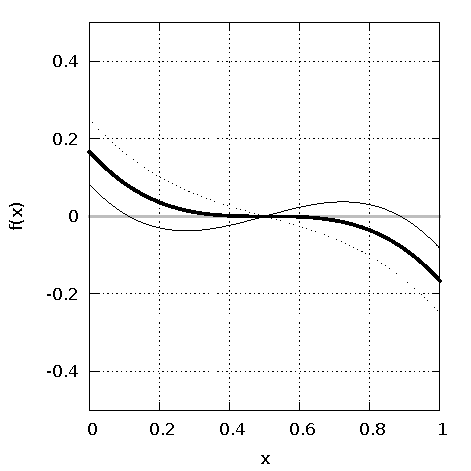
\includegraphics[width=.4\textwidth]{figure-2}
%
%\captionsetup{margin=10pt,font=small,labelfont=bf,width=.42\textwidth}

%% --- appendices ------------------------------------------------------
%\appendix
%
%% ---------------------------------------------------------------------
%\clearpage
%\section{Appendix: Some important stuff}
%
%This appendix contains all the necessary important stuff, blah, blah, blah ...
%
%\begin{landscape}
%{\footnotesize
%\begin{longtable}{lll}
%\caption{Tutaj jest tytuł tablicy}\label{tab:nowatablica1}\\
%\hline
%Nazwa atrybutu & Wartości & Opis \\ 
%\hline
%\endfirsthead
%\multicolumn{3}{c}%
%{\tablename\ \thetable\ -- \textit{kontynuacja z poprzedniej strony}} \\
%\hline
%Nazwa atrybutu & Wartości & Opis \\
%\hline
%\endhead
%\hline \multicolumn{3}{r}{\textit{kontynuowane na następnej stronie}} \\
%\endfoot
%\hline
%\endlastfoot
%chk\_acct & - & stan środków na rachunku bieżącym (jakościowa)\\ 
% & A11 & ... \textless 0 Marek Niemieckich\\  
% & A12 & 0 \textless ... \textless 200 Marek Niemieckich\\  
% & A13 & ... \textgreater 200 Marek Niemieckich\\  
% & A14 & brak rachunku bieżącego\\  
%duration & - & czas trwania kredytu w miesiącach (numeryczna)\\  
%history & - & przeszłość kredytowa (jakościowa)\\  
% & A30 & brak kredytów w historii/wszystkie kredyty poprawnie spłacone\\  
% & A31 & wszystkie kredyty poprawnie spłacone (zaciągnięte w tym banku)\\  
% & A32 & kredyty poprawnie spłacane po dzień dzisiejszy\\  
% & A33 & opóźnienia w poprzednich spłatach kredytu\\  
% & A34 & konto krytyczne/zaciągnięte kredyty w innych bankach\\  
%purpose & - & cel (jakościowa)\\  
% & A40 & nowy samochód\\  
% & A41 & używany samochód\\  
% & A42 & meble\\  
% & A43 & telewizor\\  
% & A44 & urządzenia gospodarstwa domowego\\  
% & A45 & remont\\  
% & A46 & edukacja\\  
% & A47 & wakacje\\  
% & A48 & przekwalifikowanie\\  
% & A49 & biznes\\  
% & A410 & inne\\  
%amount & - & kwota kredytu (numeryczna)\\  
%say\_acct & - & saldo na rachunku oszczędnościowym/wartość posiadanych obligacji (jakościowa)\\  
% & A61 & ... \textless100 Marek Niemieckich\\  
% & A62 & 100 \textless= ... \textless 500 Marek Niemieckich\\  
% & A63 & 500 \textless= ... \textless 1000 Marek Niemieckich\\  
% & A64 & ... \textgreater= 1000 Marek Niemieckich\\  
% & A65 & nieznane/ brak oszczędności\\  
%employment & - & czas zatrudnienia w obecnej pracy (jakościowa)\\  
% & A71 & brak zatrudnienia\\  
% & A72 & ... \textless 1 rok\\  
% & A73 & 1 \textless= ... \textless 4 lata\\  
% & A74 & 4 \textless= ... \textless 7 lat\\  
% & A75 & ... \textgreater= 7 lat\\  
%install\_rate & - & wielkość raty jako procent rozporządzalnego przychodu (liczbowa)\\  
%pstatus & - & płeć i stan cywilny (jakościowa)\\  
% & A91 & mężczyzna; rozwodnik/w separacji\\  
% & A92 & kobieta; rozwiedziona/ w separacji/ mężatka\\  
% & A93 & mężczyzna ; wolny\\  
% & A94 & mężczyzna ; żonaty/ wdowiec\\  
% & A95 & kobieta ; wolna\\  
%other\_debtor & - & inni dłużnicy/ poręczyciele (jakościowa)\\  
% & A101 & brak\\  
% & A102 & współkredytobiorca\\  
% & A103 & poręczyciel\\  
%property & - & własność/ mienie (jakościowa)\\  
% & A121 & nieruchomość\\  
% & A122 & (jeśli nie A121) umowa oszczędnościowa/ ubezpieczenie na życie\\  
% & A123 & (jeśli nie A121/A122) samochód lub inne\\  
% & A124 & nieznane\\  
%timer\_resid & - & czas zamieszkania w aktualnym miejscu zamieszkania (liczbowa)\\  
%age & - & wiek w latach (liczbowa)\\  
%other\_install & - & inne zobowiązania ratalne (jakościowa)\\  
% & A141 & bank\\  
% & A142 & sklepy\\  
% & A143 & brak\\  
%housing & - & warunki mieszkaniowe (jakościowa)\\  
% & A151 & wynajem\\  
% & A152 & własność\\  
% & A153 & zamieszkanie bez ponoszenia kosztów\\  
%other\_credits & - & liczba aktualnych kredytów w tym banku (liczbowa)\\  
%job & - & praca (jakościowa)\\  
% & A171 & bezrobotny/niewykwalifikowany; cudzoziemiec\\  
% & A172 & niewykwalifikowany; rezydent\\  
% & A173 & wykwalifikowany pracownik/urzędnik\\  
% & A174 & menadżer/ samozatrudniony/ wysocewykwalifikowany/ wyższy urzędnik\\  
%num\_depend & - & liczba osób na utrzymaniu (liczbowa)\\  
%telephone & - & telefon (jakościowa)\\  
% & A191 & brak\\  
% & A192 & tak, zarejestrowany pod nazwiskiem klienta\\  
%foreign & - & pracownik zagraniczny (jakościowa)\\  
% & A201 & tak\\  
% & A202 & nie\\  
%response & - & decyzja kredytowa\\  
% & 1 & tak\\  
% & 2 & nie\\ 
% \hline
%\end{longtable}}
%\end{landscape}
%


% --- bibliography ----------------------------------------------------
\clearpage
\bibliographystyle{agsm}
\bibliography{refs}

% --- abstract --------------------------------------------------------
\clearpage
\addcontentsline{toc}{section}{List of tables}
\listoftables

% --- abstract --------------------------------------------------------
\clearpage
\addcontentsline{toc}{section}{List of figures}
\listoffigures



% --- abstract --------------------------------------------------------
\clearpage
\addcontentsline{toc}{section}{Streszczenie}
\section*{Streszczenie}

Tutaj zamieszczają Państwo streszczenie pracy. Streszczenie powinno być długości około pół strony.


\end{document}


%%% Local Variables:
%%% mode: latex
%%% TeX-master: t
%%% End:
